\section{Radiation Shielding Infrastructure}

\subsection{Space Radiation}

On Earth, a significant portion of the radiation humans receive \cite{lamarsh} are from terrestrial source (radioactive nuclides found on Earth) and man-made source like medical procedures, air travel, tobacco, etc. Radiation can also be received sources outside of Earth, but these are normally attenuated by the atmosphere. In space however, extraterrestrial and non-man-made sources are far more important. When designing spacecraft, it is the extraterrestrial sources that are modeled.

Extraterrestrial radiation sources take three forms, all of which are represented in Fig. \ref{fig:space-radiation}. The dominant radiation source comes from galactic cosmic rays (GCRs). These rays consist of almost entirely protons and other heavy ions with energies up to trillions of MeV. These heavy ions pose a great threat to astronauts because of their high penetration. Since GCRs contain a broad list of heavy charged ions, relative abundances can be determined as seen in Fig. \ref{fig:abundances}. Radiation in space can also be received from Earth’s trapped radiation belts (ERBs) where charged particles are kept in the vicinity of Earth by the complex rotations of Earth, its gravitational field, and the surrounding solar system. Finally, radiation also comes in the form of emissions from the Sun.

While several man-made sources are concerning to humans living on Earth, space radiation is arguably more dangerous considering the energy and intensity received even at low earth orbit (LEO). In fact, it is evident that astronauts exhibit higher risks of diseases and cancers that can be the result of increased radiation exposure in space \cite{nature-apollo}. Earth’s atmosphere serves as a strong shielding system against GCRs and radiation from the Sun. However, in space, this thick atmosphere of gases and molecules are absent to protect astronauts. Instead, shields must be designed that block sufficient amounts of space radiation to maintain the health of humans sent to space.

Career limits for occupations exposed to radioactivity are defined by the National Council on Radiation Protection and Measurements (NCRP). Limits for astronauts rely heavily on dosimetry measurements recorded during space exploration like the NASA shuttle missions of the 20th century \cite{cucinotta-shuttle}. The NCRP recommended LEO career limits up to 4 Sv depending on age and sex in their Report No. 132 \cite{ncrp-132}. This limit is notably higher than the accepted occupational exposure for radiation workers on Earth of 2.5 Sv (5 rem per year for a 50-year work-life \cite{lamarsh}). The limit is higher because the exposure is inevitably higher in space than on Earth. Even though the limit is higher, significant work has been done to ensure the career limit does not pose dangerous increases in the risk of developing cancer. This is a difficult estimation to make but its uncertainty is often determined using simulations like Monte Carlo to produce probability distribution functions (PDFs) \cite{cucinotta-pdf}.

In abiding with these radiation limits, shielding structures are designed by considering the cascading effects of GCRs (and other space radiation) and the interactions with structural materials. The different interactions are detailed in Fig. \ref{fig:shield-transport}. This should demonstrate that the expansive interaction mechanisms result careful consideration of all materials use in a spaceship. While on Earth lead is commonly used to shield again radiation, aluminum is favored on spacecraft for its light and economically efficient shielding of radiation. However, shield engineering does not stop at designing the spacecraft because astronauts conduct extra-vehicular activities (EVAs) like spacewalks where equipment like spacesuits and lunar buggies need to be designed to limit radiation exposure. Again, doses are commonly estimated using probability modeling of different shielding scenarios until an adequate shielding thickness is determined \cite{eva-model}.

\begin{figure}
\centering
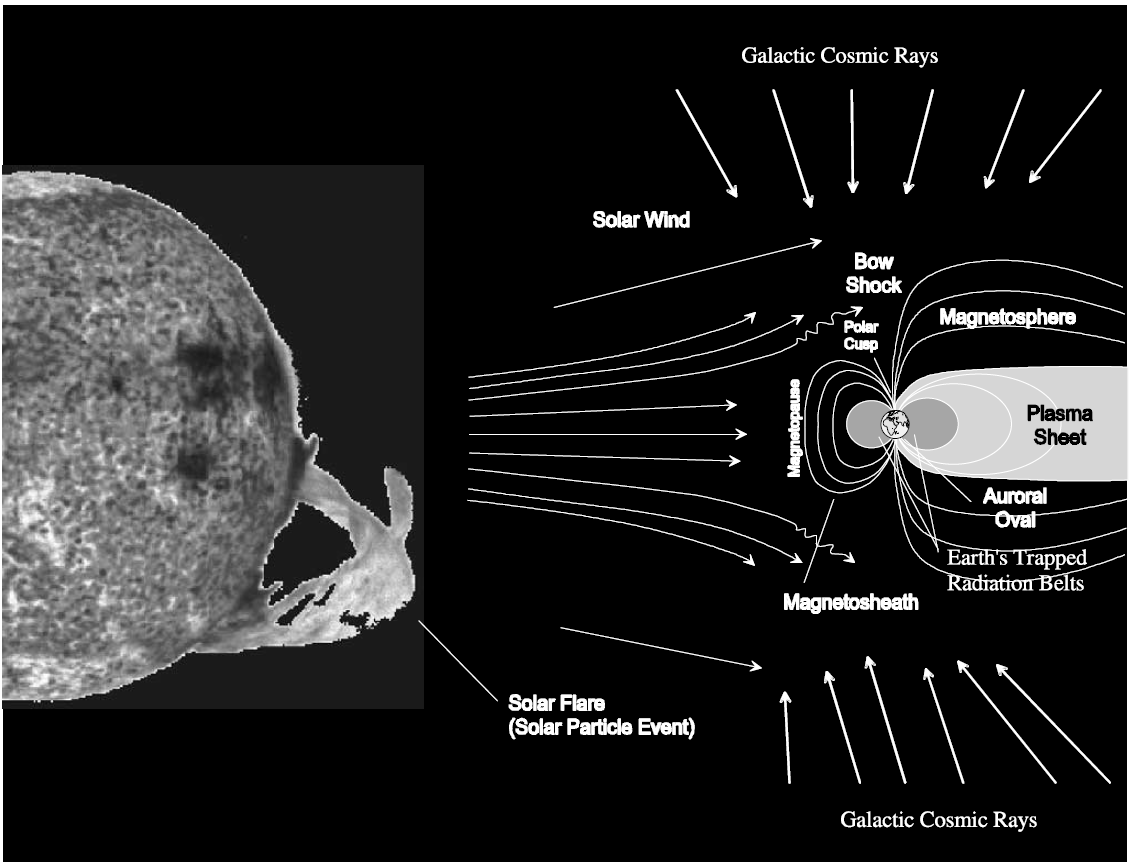
\includegraphics[scale=0.5]{space_radiation.png}
\caption{Characteristic extraterrestrial radiation as presented by \cite{bentonbenton}. Radiation doses in space are received from three sources: galactic cosmic rays (GCRs), radiation trapped in Earth’s radiation belt (ERBs), and charged particles produced and emitted by the Sun. Collectively these sources need to be considered when designing spacecraft shielded enough to protect astronauts who use them.}
\label{fig:space-radiation }
\end{figure}

\begin{figure}
\centering
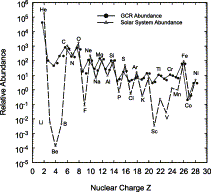
\includegraphics[scale=0.5]{abundances}
\caption{Relative abundances of galactic cosmic rays received in space \cite{bentonbenton}. These heavy charged nuclei pose a threat to astronauts due to their penetrative nature and high energies.}
\label{fig:abundances }
\end{figure}

\begin{figure}
\centering
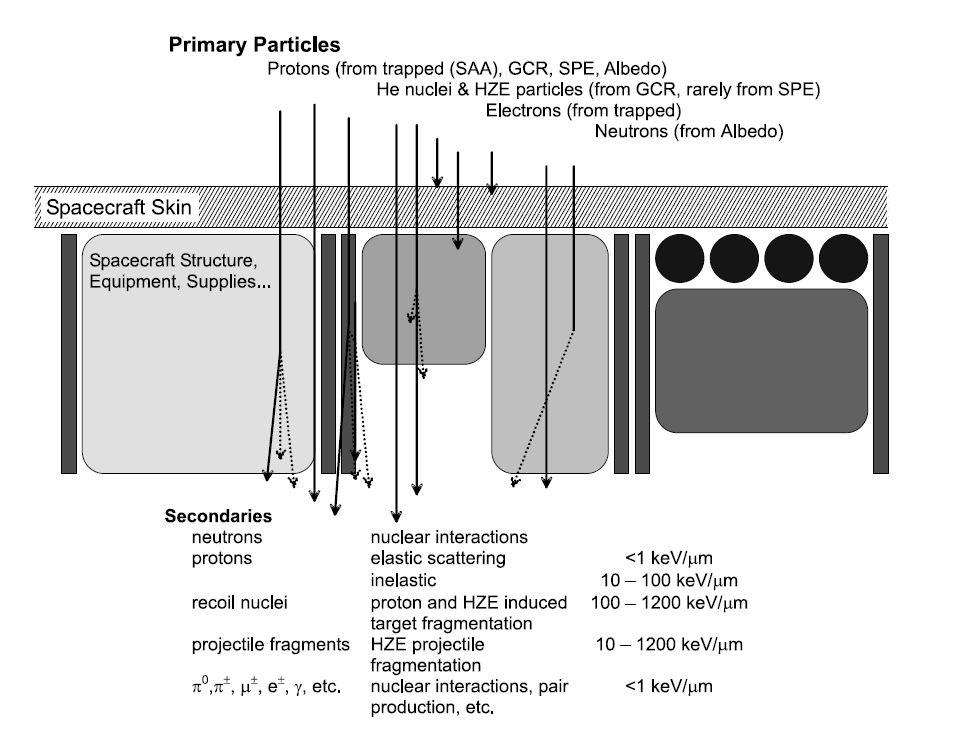
\includegraphics[scale=0.5]{shield_transport.png}
\caption{Generalized diagram of radiation interactions with spacecraft materials \cite{bentonbenton}. Radiation from different extraterrestrial sources has different penetrating properties that can potentially be deposited deep into a spacecraft where shielding is not adequate and can result in lower energy secondary radiation that also needs to be blocked.}
\label{fig:shield-transport }
\end{figure}

\subsection{The International Space Station}

The difficulty with quantifying radiation exposure in space is the lack of experimental data. On Earth, it is accessible to obtain radiation measurements either through probes/sensors or controlled experiments. Taking measurements in space requires sending satellites that can be costly investments in an extremely fragile environment. Slowly over the years, data has been collected as space missions became more complex. Only two scenarios have seen humans live in space: manned missions to the moon and LEO missions. Certainly humans have more experience with LEO since the completion of the International Space Station (ISS): a permanently habituated artificial satellite operating in LEO for two decades.

In order to design the ISS, some estimation of the expected radiation dose in LEO was required. This was accomplished with dosimetry data collected from NASA shuttle flights \ref{cucinotta-shuttle} \ref{ohnishiohnishi} \ref{mccormack}. With some baseline achieved, modeling could be completed that formed as low as reasonably achievable (ALARA) radiation doses. The preferred shielding material has been polyethylene (plastic) or water, which is favorably lightweight for manned missions \ref{alara}. Interestingly, mission duration to the ISS tends to be limited to under a year because, even with shielding, doses are high enough to become a threat for long periods of exposure.

Throughout the lifetime of the ISS, estimations of radiation exposure have improved. Since astronauts have been meticulously monitored over the years, scientists have been able to more accurately determine probability of cancer risks and fatalities for varying mission lengths on the ISS \ref{cucinotta-cancer}. Under the guidance of NASA, countermeasures (like shielding and length of stay) attempt to limit radiation exposure so that the increased fatality due to cancer does not increase for astronauts more than 3\% at a 95\% confidence interval. New advances in technology have also helped to improve living conditions in space. For example, Kevlar has seen increased interest as a material to protect against meteoroids and debris. In fact, Kevlar has demonstrated favorable radiation shielding properties as well and may be a valuable substitute for common shielding materials like polyethylene and aluminum \ref{accelerators}. All the data collected at the ISS and research conducted therein are important precursors to more ambitious manned missions. Unfortunately, despite being a space operation, LEO missions are not entirely informative to the conditions exhibited in deep space. For manned missions to Mars to be successful, missions out of Earth’s immediate vicinity need to conducted first. This has led to revived interest in moon landing missions. The last moon landing was Apollo 17 in 1972. The advent of more advanced technology in the 40 years since that mission necessitates a reevaluation of the limited radiation data collected during the Apollo missions.
